\documentclass[12pt]{article}\usepackage[]{graphicx}\usepackage[]{color}
% maxwidth is the original width if it is less than linewidth
% otherwise use linewidth (to make sure the graphics do not exceed the margin)
\makeatletter
\def\maxwidth{ %
  \ifdim\Gin@nat@width>\linewidth
    \linewidth
  \else
    \Gin@nat@width
  \fi
}
\makeatother

\definecolor{fgcolor}{rgb}{0.345, 0.345, 0.345}
\newcommand{\hlnum}[1]{\textcolor[rgb]{0.686,0.059,0.569}{#1}}%
\newcommand{\hlstr}[1]{\textcolor[rgb]{0.192,0.494,0.8}{#1}}%
\newcommand{\hlcom}[1]{\textcolor[rgb]{0.678,0.584,0.686}{\textit{#1}}}%
\newcommand{\hlopt}[1]{\textcolor[rgb]{0,0,0}{#1}}%
\newcommand{\hlstd}[1]{\textcolor[rgb]{0.345,0.345,0.345}{#1}}%
\newcommand{\hlkwa}[1]{\textcolor[rgb]{0.161,0.373,0.58}{\textbf{#1}}}%
\newcommand{\hlkwb}[1]{\textcolor[rgb]{0.69,0.353,0.396}{#1}}%
\newcommand{\hlkwc}[1]{\textcolor[rgb]{0.333,0.667,0.333}{#1}}%
\newcommand{\hlkwd}[1]{\textcolor[rgb]{0.737,0.353,0.396}{\textbf{#1}}}%
\let\hlipl\hlkwb

\usepackage{framed}
\makeatletter
\newenvironment{kframe}{%
 \def\at@end@of@kframe{}%
 \ifinner\ifhmode%
  \def\at@end@of@kframe{\end{minipage}}%
  \begin{minipage}{\columnwidth}%
 \fi\fi%
 \def\FrameCommand##1{\hskip\@totalleftmargin \hskip-\fboxsep
 \colorbox{shadecolor}{##1}\hskip-\fboxsep
     % There is no \\@totalrightmargin, so:
     \hskip-\linewidth \hskip-\@totalleftmargin \hskip\columnwidth}%
 \MakeFramed {\advance\hsize-\width
   \@totalleftmargin\z@ \linewidth\hsize
   \@setminipage}}%
 {\par\unskip\endMakeFramed%
 \at@end@of@kframe}
\makeatother

\definecolor{shadecolor}{rgb}{.97, .97, .97}
\definecolor{messagecolor}{rgb}{0, 0, 0}
\definecolor{warningcolor}{rgb}{1, 0, 1}
\definecolor{errorcolor}{rgb}{1, 0, 0}
\newenvironment{knitrout}{}{} % an empty environment to be redefined in TeX

\usepackage{alltt}
%Required: You must have these
\usepackage{graphicx}
\usepackage{tabularx}
\usepackage{natbib}
\usepackage{pdflscape}
\usepackage{array}
\usepackage{authblk}
\usepackage{gensymb}
\usepackage{amsmath}
%\usepackage[backend=bibtex]{biblatex}
\usepackage[small]{caption}

\setkeys{Gin}{width=0.8\textwidth}
\setlength{\captionmargin}{30pt}
\setlength{\abovecaptionskip}{10pt}
\setlength{\belowcaptionskip}{10pt}

 \topmargin -1.5cm 
 \oddsidemargin -0.04cm 
 \evensidemargin -0.04cm 
 \textwidth 16.59cm
 \textheight 21.94cm 
 \parskip 7.2pt 
\renewcommand{\baselinestretch}{1.6} 	
\parindent 0pt
\usepackage{setspace}
\usepackage{lineno}

\bibliographystyle{..//..//sub_projs/refs/styles/besjournals.bst}
\usepackage{xr-hyper}
%\usepackage{hyperref}
\externaldocument{SUPP_FLS_flobud}
\externaldocument{JOErev_resp_parII}
\title{Differences between flower and leaf phenological responses to environmental variation drive shifts in spring phenological sequences of temperate woody plants}
\date{}
\author{D.M. Buonaiuto $^{1,2,a}$, E.M. Wolkovich$^{3}$}
\IfFileExists{upquote.sty}{\usepackage{upquote}}{}
\begin{document}
\maketitle
\noindent \emph{Author affiliations:}\\
\noindent $^1$Arnold Arboretum of Harvard University, Boston, Massachusetts, USA. ORCID: 0000-0003-4022-2591\\
$^2$Department of Organismic and Evolutionary Biology, Harvard University, Cambridge, Massachusetts, USA \\
$^3$Forest \& Conservation Sciences, Faculty of Forestry, University of British Columbia, Vancouver, British Columbia, Canada\\
$^a$Corresponding author: 617.823.0687; dbuonaiuto@g.harvard.edu\\
\pagebreak


\maketitle
\linenumbers
\section*{Abstract} 
The relative timing of growth and reproduction is an important driver of plant fitness. For deciduous woody species in temperate regions leaves and flowers both appear in the early spring, but the order and duration of these phenological events vary among species, populations, and individuals. \linelabel{ab1} Researchers have long hypothesized that this variation in flower-leaf sequences (FLSs) may be important---affecting the reproduction, recruitment and survival of individuals. Further,  FLSs appear to be shifting with climate change; thus anticipating the extent of these shifts may influence projections of how climate change may impact species' performance and reshape forest communities. Predicting\linelabel{abs2} FLS shifts requires an improved understanding of how environmental variation dictates FLS patterns. To address this, we compared the phenological responses of flowers and developing leaves for 10 temperate woody species to varying levels of temperature and photoperiod in a lab experiment. Our experimental design allowed us to test competing hypotheses for how environmental cues determine FLS variation---specifically whether forcing (warm temperatures) alone drives variation or differential sensitivity to chilling (cool temperatures generally in the fall and winter) and/or photoperiod matter. Within\linelabel{abs3} species, we found that flower and leaf phenology responded with differential sensitivity to environmental cues, with differences in their response to chilling being the dominant driver of FLS variation. These differences\linelabel{sults1} between flowering and leaf responses were consistent across species, but because species differ the order of phenological events in their FLSs (flowering-first vs. leafing-first), differences between flower and leaf phenology will have contrasting impacts on FLS variation across species. Because climate change will amplify variability in chilling across time and space, our findings suggest that FLS shifts may be large, but are likely to vary substantially among populations and\linelabel{abs4} species. Simple projections of FLS shifts with climate change, based on our results, showed large shifts in wind-pollinated species that flower before leafing, with flower-leaf interphases substantially shortened. This shorter interphase would reduce the time period for efficient
pollen transfer, and thus raises the possibility that wind-pollinated
taxa especially may experience reproductive declines due to FLS shifts
in the decades to come.

%When we projected how FLSs are likely to shift under several generalized climate change scenarios, we found that FLS shifts were largest in wind-pollinated species that flower before leafing, with flower-leaf interphases substantially shortened under all scenarios. This flower-leaf interphase is critical for effective pollen transfer in wind-pollinated taxa, and the direction and magnitude of shifts we found for these species raises the possibility that, more generally, wind-pollinated taxa may experience reproductive declines due to FLS shifts in the decades to come.   \\ % 344 words out of 350 permitted

\noindent \emph{Keywords:} chilling, climate change, deciduous forests, flower-leaf sequences, forcing, hysteranthy, phenology, wind-pollination  \\ 

\section*{Introduction}
\noindent Among the most widely documented biological effects of anthropogenic climate change are shifts in plant phenology, the timing of life cycle events \citep{Parmesan2003,Menzel2006,Cleland2007}. While phenology is generally advancing with climate change, the strength of these phenological shifts can vary substantially among specific phenological phases \citep{Augspurger:2020aa}. These differences alter the timing of phases relative to each other, changing the duration between events that make up phenological sequences \citep{Ettinger2018}. Phenological sequences are a major driver of plant fitness that impact plant life history, resource allocation, demography and ecosystem processes \citep{Post:2008aa}. Thus, shifting sequences with climate change will likely impact many of these processes. The effects of these shifts, however, depend both on their direction---whether distinct phases are shifting closer together or farther apart---and magnitude---how much they are shifting relative to each other.\\ 

\noindent \noindent For deciduous woody plants, the relative timing of flower and leaf phenology, or flower-leaf sequences (FLSs), may be particularly consequential to fitness in temperate regions where flowering prior to leaf development is common \citep{Rathcke_1985}. There are several hypotheses regarding the function of FLS variation \citep[see][]{Gougherty2018}, and it is likely that the adaptive significance of FLSs vary among species, and may co-vary with other plant traits.\\

\noindent The flowering-first FLS is strongly correlated with wind-pollination \citep{Buonaiuto2020, Friedman2009} and models of pollen movement\linelabel{wind1} show that for wind-pollinated species, flowering-first increases pollen dispersal distances and significantly reduces the amount of pollen intercepted by non-reproductive structures \citep{Di-Giovanni:1989aa,Tauber1967,Whitehead1969}. Flowering-first is also prevalent in some biotically-pollinated taxa, but its function is less clear. Some authors suggest that flowering-first impacts floral visibility to pollinators \citep{Janzen1967, Bukovac:2017aa,Forrest:2009aa} or modifies hydraulic demand \citep{Gougherty2018,Franklin2016}, while, others suggest that in biotically-pollinated taxa there is no unique function to the sequence and flowering-first a by-product of selection for early flowering in general \citep{Primack1987}.\\ 

\noindent Phenological observations over the last several decades indicate that, like other phenological sequences, FLSs are shifting with climate change \citep{Ma2020:aa}. For several species, the time between flowering and leafing appears to be increasing, but the strength of this trend varies among species and the direction of FLS shifts are not consistent across populations \citep{Buonaiuto2020,Ma2020:aa}. These changes could affect the important functions of FLSs, potentially putting some species at greater risk for fitness declines, while benefiting others.\\

%However, the functional significance of FLS variation may depend on other species traits such as pollination syndrome or drought tolerance \citep{Gougherty2018}. \\

%\noindent While the function of FLS variation may vary among species, flowering-first is a risky strategy. Flowering-first species must begin their reproductive investment from stored carbohydrates alone, at a time of year when these reserves at are their lowest \citep{Primack1987}, and the risk of damage from late-season frost is highest \citep{Zohner2020}, and it is becoming clear that the costs of this tradeoff may be shifting due to anthropogenic climate\linelabel{wind2} change.\\  %EMW24Mar2021: If you keep the re-order, slightly tweak this transition. Also, "it is becoming clear that" is too wordy -- re-order or rephrase this clause. 

\noindent The impact\linelabel{wind3} on FLS shifts with climate change on the fitness of woody plants depends on 1) the function of FLS for that species and 2) the direction and magnitude of the shift. For example, in wind-pollinated species that rely on a substantial flower-leaf interphase for effective pollen transport, decreasing FLS interphases with climate change may drive a reduction in pollination success as more pollen is intercepted by vegetation. Conversely, pollination efficiency could improve for species with lengthening FLS interphases. However, a proportionate FLS shift in biotically-pollinated taxa may have different fitness implications because the contrasting function of FLS variation in these species\linelabel{wind4}.\\
%DMB March 30 This was a bone for reviewer one, but I am worried there is no way to go into enough detail here without extending teh conversation tooo.


\noindent While several recent analyses have examined the function of FLS variation \citep[e.g.][]{Buonaiuto2020, Gougherty2018}, the factors that influence the magnitude and direction of FLS shifts are less well studied  \citep[but see][]{Ma2020:aa}. Predicting FLS shifts requires identifying the proximate mechanisms that drive and constrain FLS variation, and how these mechanisms differ among species.\\
 
\noindent Decades of research suggest that cool winter temperatures (chilling), warm spring temperatures (forcing), and day-length (photoperiod) are the primary drivers of both reproductive and vegetative phenology  for woody plants in temperate regions \citep{Korner:2010aa,Flynn2018}. However, observed FLS shifts indicate that there must be differences in how these cues influence the phenology of flowers and leaves \citep{Buonaiuto2020}.

\noindent It\linelabel{buds1} is also likely that FLS variation is mediated by other internal mechanisms like developmental construction \citep{Diggle1995}, or other physical constraints like inflorescence architecture or bud type \citep{Pope2013}. For example, FLS variation in species with separate buds (buds containing either embryonic leaves or flowers) may be less constrained than species with mixed buds (buds containing both embryonic leaves and flowers together). Other factors like\linelabel{shrub} growth form (tree vs. shrub) or colonization-competition tradeoffs that have been show to influence the phenological sensitivity of specific phenophases \citep{Basler:2012aa,Donnelly:2021aa} may also influence the sensitivity of phenological sequences to climate\linelabel{buds2}.\\

\noindent While FLS variation in woody plants is no doubt the product of interactions between species-specific biology and complex environmental inputs, identifying the differences in how flower and leaf phenology responds to environmental change is a necessary step for predicting the direction, magnitude and---ultimately---fitness impacts of FLS shifts with climate change. Studies that have attempted to identify the differences between reproductive and vegetative phenology in woody plants (mostly focused on crop species) have yielded two common explanations which we present below.

\subsection*{Hypotheses for FLS variation}

\noindent One hypothesis suggests that reproductive and vegetative buds utilize the same underlying environmental cues, but have different threshold responses to forcing, with whichever bud type bursts later---leaves or flowers---having a higher thermal requirement \citep[that is, they need a greater sum of warm temperature to trigger the phenological event,][]{Guo2014,COSMULESCU:2020aa,Cosmulescu:2018aa}. Under this hypothesis, which we call the forcing hierarchy hypothesis (FHH), leaf and flower buds share the same suite of cues and develop similarly to non-forcing cues (i.e., chilling and photoperiod), but differ in the thermal requirement for budburst.\\

\noindent In contrast, an alternative hypothesis suggests that flower and leaf buds differ in the strength of their phenological responses to multiple environmental cues \citep{Citadin2001,Gariglio2006,Aslani2009,Mehlenbacher:1991aa}. Under this hypothesis, which we call the differential sensitivity hypothesis (DSH), each bud type relies more or less on certain cues, generating FLS variability.\\ 

\noindent While observational studies of phenology in the field are commonly used to evaluate the relationship between environmental conditions and phenology \citep{Cleland2007}, under current and recent climatic conditions, the FHH and DSH may produce similar phenological patterns, making it difficult to evaluate these hypotheses with such methods. However, experiments designed to isolate all three environmental cues have the potential to disentangle the two hypotheses. Studies aiming to differentiate these hypotheses can look for two different signatures. The key signature of the FHH is that the sensitivity to forcing ($\Delta$ day of phenological event/ $\Delta$\degree C) of the second phase in the phenological sequence is always greater than that of the first phase with sensitivity differences being inversely proportional to the difference in thermal requirement among bud types (2x in our simulations; Fig. \ref{fig:simulations} a.). By contrast, the signature of the DSH is that sensitivity estimates of flower and leaf buds to chilling and/or photoperiod will diverge (Fig. \ref{fig:simulations} b.), but there is no characteristic pattern as to the strength or direction of this divergence (e.g., leaves may require longer or shorter photoperiods than flowers, or more or less chilling).\\


\noindent The clarity of these signatures from each hypothesis, however, may be obscured in certain situations. First, a species' buds could be both differentially sensitive to photoperiod or chilling (supporting the DSH) and also respond to forcing in a forcing hierarchy (that is, both hypotheses can operate at once, see Fig. \ref{fig:simulations} c.). Second, the differential sensitivity framework can generate the signature of the FHH when other cues are at high levels due to interactions between the chilling or photoperiod response and the thermal requirement, which make forcing the dominant phenological cue once other cue requirements have been met (see Fig. \ref{fig:simulations} b., chill x force interaction). When this happens the FHH would effectively be a special case of the DSH.\\ 

\noident While these two hypothesized mechanisms may produce similar phenology patterns under current conditions, differentiating them %, and understanding if they are generally separate in nature, 
is important, as they have substantially different implications regarding the potential for FLS shifts with climate change. The FHH suggests that FLS variation is largely a product of climate variation during the interphase. If spring temperatures increase with climate change, the second phenophase of the FLS will be accelerated relative to the first and FLS interphases will decrease, but given the relative auto-correlation of spring temperatures \citep{Di-Cecco:2018aa}, these shifts should be muted. If FLSs are structured by a forcing hierarchy, the direction of FLS shifts are relatively straight forward to predict, and it is less likely that shifts will be large enough in magnitude to significantly affect woody plant fitness.\\

\noindent Climate change would also drive FLS shifts under the DSH, but the trajectory of these shifts are more complicated to predict. The DSH suggests that there could be\linelabel{reg} strongly localized or regional effects of climate change on FLSs. Shifts in FLS variation will depend on the direction and rate of change in cues at given locations and the species-specific differential sensitivity of reproductive and vegetative phenology to cue combinations. This hypothesis allows for larger magnitude shift in FLSs, on a scale that could impact pollen transport or the physiological functioning of woody plants. Further, the DSH also suggests that the magnitude of shifts may be highly divergent both among species in a community, and among populations of the same species which could impact gene flow, population structure and demography.\\

\noindent In this study we tested the FHH and DSH hypotheses in 10 temperate shrub and tree species. Using a full-factorial growth-chamber experiment we manipulated chilling, forcing and photoperiod cues for flower and leaf buds. We then leveraged these data to examine how FLSs may shift with climate change.\\ % to identify species' characteristics associated with high magnitude FLS shifts

\section*{Materials and Methods}

\subsection*{Growth chamber study}

\noindent We sampled plant material from Harvard Forest in Petersham, MA, USA (42.5314\degree N, 72.1900\degree W) on 25 October 2017, just as most individuals dropped their leaves\linelabel{harvest}, to capture the period immediately after most plants in the area entered endo-dormancy but before they could accumulate significant chilling in the field. We collected branch cuttings from 7-13 individuals of 12 woody plant species (4-12 cuttings per individual for a total of 48-56 per species), consisting of a mix of deciduous shrubs, understory and canopy trees commonly found in mesic hardwood forests of the eastern United States. The use of branch cuttings to study woody plant phenology in artificial environments is common \citep{Ettinger:2020aa}, and these methods have been shown to match whole-plant phenological patterns  \citep{Vitasse:2014aa,Primack2015}.
We\linelabel{criteria1} selected species displaying variation of the three major FLS patterns; species for which flowers appear before leaves (flowering-first; \textit{Acer rubrum}, \textit{Betula alleghaniensis}, \textit{Comptonia peregrina}, and \textit{Corylus cornuta}), species for which flowers appear with their leaves (concurrent; \textit{Acer pensylvanicum}, \textit{Acer saccharum}, \textit{Ilex mucronata}, \textit{Prunus pensylvanica}, \textit{Vaccinium corymbosum}), and species for which flowers appear after leaf development (leafing-first; \textit{Ilex verticillata}, \textit{Prunus virginiana}, \textit{Viburnum acerifolium}). Because we\linelabel{traits1} expected that other characteristics such as pollination syndrome, bud type, and growth habit were likely to impact FLS sensitivity, we made sure that the species we chose exhibited variation in these traits as well  (see Tab. \ref{tab:splist} for details and full species list). \linelabel{phylo1} We included several congenerics in our study, explicitly choosing species with different FLS patterns (which therefore could not have been inherited from a common ancestor) to mitigate phylogenetic non-independence in\linelabel{phylo2} our trait of interest (FLS) \citep{Revell:2010aa}.\\
%EMW24Mar2021: I don't think 'while' is the right word here -- the presence of congenerics strengthens the experiment

We transported all cuttings to the Arnold Arboretum in Boston, MA (USA) where they were re-cut in water to prevent callousing and minimize\linelabel{embolism} embolism and placed in 500 ml Erlenmeyer flasks with distilled water.\\ 

\noindent We randomly assigned cuttings to a fully crossed set of eight experimental treatments; two levels of chilling (4 vs 8 weeks at 4\degree C), two levels of temperature (24\degree C:18\degree C (day/night) warm vs 18\degree C:12\degree C (day/night) cool) and two levels of photoperiod (12 vs 8 hours). We alternated day/night temperature periodicity on a 12 hour schedule to reduce co-variation with photo-periodicity. We re-cut all twigs and changed the water every 7-10 days and rotated all treatments between growth chambers every two weeks to minimize chamber effects. We made phenological observations every 2-3 days using a modified BBCH scale for woody plants \citep{Finn2007} for three months following release from chilling conditions. In this period we assessed three phenological phases: leaf budburst (BBCH phase 07), leafout (BBCH phase 15) and first flower open (BBCH 60). While\linelabel{caveat1} leaf budburst is the first stage of vegetative expansion and therefore most directly comparable to first flowering, we also included leafout in our observations because several of the functional hypotheses for FLS variation are predicated on developing leaves be sufficiently large enough to impact canopy structure, which would only happen at later stages of leaf development.\\ 

\noindent At the conclusion of this period we assessed all individuals that did not undergo budburst and excluded 56 dead twigs from our analyses. 

\subsection*{Data analysis}

\noindent To assess the phenological sensitivity of each phase, we fit mixed-effects hierarchical models with chilling, forcing, photoperiod and all two-way interactions as the fixed effects and species as a grouping factor on both the slopes and the intercepts. We chose a Bayesian hierarchical approach in order to identify systematic trends across species' responses while accounting for sample size, variance, and the unique effect of each species. %We also standardized the units of each environmental predictor to allow for appropriate comparisons between them \citep{Gelman2007}. 
We modeled the effects of environmental parameters on flower opening, leaf budburst and leafout separately. We also fit a model with FLS interphase (day of budburst - day of flowering) as a response variable to compare these estimates with field observations. Two species, \textit{Betula allegheniensis} and \textit{Acer saccharum}, produced no flowers in our trial, likely because flowering branches were out of reach during our field sampling, so we excluded them from our analysis. In total, our analyses included 464 twigs from 10 species. \\ 

The models we fit appear below:\\

$y_{[i]} \sim N(\alpha_{sp_{[i]}}+\beta_{forcing_{sp[i]}}+\beta_{chilling_{sp[i]}}+\beta_{photoperiod_{sp[i]}}+\beta_{forcing x chilling_{sp[i]}}+\beta_{forcing x photoperiod_{sp[i]}}+\beta_{chilling x photoperiod_{sp[i]}}, \sigma_y^2)$\\

Where $y_{[i]}$ is either the day of the experiment of leaf budburst, day of first flower opening, day of leafout or FLS interphase length, and $\sigma_y^2$ the error.  We modeled the intercept ($\alpha$) and each slope ($\beta$) parameter at the species level using the formula:\\

$\alpha_{x_{sp}} $or $\beta_{x_{sp}} \sim N(\mu_x,\sigma^2_x)$\\

\noindent To test the hypothesis that the FHH is a special case of the DSH that occurs when other cue (i.e., chilling and photoperiod) requirements are met, we re-ran our leaf budburst and flowering models on a subset of our data which included both levels of the forcing treatment but only the high photoperiod and chilling treatment levels. This model included forcing as the only main effect but, like our main models written above, included species as a grouping factor on the slopes and intercept.\\ 

\noindent We fit all models using the R package ``brms" \citep{Burkner2018}. We ran each model on four chains with 4000 iterations and a 3000 iteration warm up for a total of 4000 posterior draws for each parameter. In all models we used weakly informative priors and increasing the priors 5-fold did not affect the model results. We assessed  model performance through ensuring $\hat{R}$s were between 1 and 1.01 and bulk and tail effective sample sizes were high (1800-2800 for most parameters, but as low as  800-900 for some). We present 50\% credible intervals in figures because they are the most computationally stable \citep{Gelman2013}, but provide other intervals in the Supporting Information (Tab. \ref{tab:modelests}, Tab. \ref{tab:modelests2}, Tab. \ref{tab:phh}). All\linelabel{standard} of our estimates of phenological sensitivity ($\Delta$ day of phenological event/ $\Delta$ environmental cue) are scaled by treatment level (chilling: $\Delta$ 4 weeks, forcing: $\Delta$ 6\degree C, photoperiod: $\Delta$ 4 hours).\\

\subsection*{Climate change scenarios}
\noindent To apply our model results to general climate change scenarios we chose environmental treatments in the experiment to broadly reflect historic and future conditions at our sampling site. Our low forcing treatment approximated average spring temperature (March/April) at the site while our high temperature treatment reflects a 6 \degree C increase. Average field chilling \citep[calculated from 15 October - 15 April, measured in Chill Hours,][]{Weinberger:1950aa} at Harvard Forest is 1170.7, approximately  63\% of the difference between our low and high chilling treatment (Tab. \ref{tab:chillcomps}). Thus, our low chilling treatment represents a feasible estimate for a decrease in chilling with climate change and our high chilling treatment approximates a reasonable increase \citep{Luedeling:2012aa}. Our low photoperiod treatment (8 hours of daylight) is well below the photoperiod experienced at Harvard Forest, but given that the photoperiod effects are expected to be small \citep{Laube:2014a}, we chose more extreme values in order to robustly estimate an effect (i.e., increasing statistical power). For this reason, our climate change scenarios for FLS variation are based on our high photoperiod treatment alone.\\


\noindent We used our flower, leafout and leaf budburst models to project for each species in our study:
\begin{enumerate}
\item FLSs under average environmental conditions  (low forcing, ~6.5 weeks of chilling treatment)
\item FLS shifts with spring warming only (high forcing, ~6.5 weeks of chilling treatment)
\item FLS shifts with warming and increased chilling (high forcing, ~8 weeks of chilling treatment)
\item FLS shifts with warming and decreased chilling (high forcing, ~4 weeks of chilling treatment)
\end{enumerate}

\noindent To validate our predictions, we compared our FLS interphase model estimates of ``average" condition FLS interphases to long term phenological records from Harvard Forest \citep{OKeefe2015} for five species common to both datasets (Fig. \ref{fig:validate}), and found them comparable. \\

\noindent Given the variable dynamics of shifts in environmental forcing and chilling with climate change over time and space \citep{Luedeling:2011aa}, these scenarios should not be treated as absolute predictions of the magnitude of FLS shifts with climate change. Instead, we provide these scenarios to identify general trends in how FLSs could shift with warming and demonstrate that the range of possibilities vary based on characteristics of plant species and the specific climate dynamics.\\

\noindent Finally, we characterized FLS shifts for three broad FLS groups (flowering-first, concurrent, leafing-first) by extracting all sampling posterior estimates from our main models using the R package tidybayes \citep{Kay2020}, and grouping them by FLS pattern. We also include the species-specific estimates on which these grouped estimates are based in Fig. \ref{fig:preddy_sp}.  \\ 

\section*{Results} 
\subsection*{Growth chamber study} 
\noindent  Flowering, leaf budburst and leafout advanced with higher forcing and longer chilling duration (flowering: chilling effect: -21.2 days, forcing effect: -19 days, leaf budburst: chilling effect: -30.4 days, forcing effect: -17.8 days, leafout: chilling effect: -39.7 days, forcing effect: -32.6 days; Fig. \ref{fig:model}, Fig. \ref{fig:altview}, Tab. \ref{tab:modelests}, Tab. \ref{tab:modelests2}---all sensitivity estimates are scaled by treatments; see ``Data analysis" section above), but increases in both of these cues together offset these advances (flowering: force x chill effect: 7.0 days, leaf budburst: force x chill effect: 12.4 days, leafout: force x chill effect: 21.4 days; Fig. \ref{fig:model},Fig. \ref{fig:altview}, Tab. \ref{tab:modelests}, Tab. \ref{tab:modelests2}). Leaf and flower phenologies diverged in their responses to photoperiod, with flower phenology advancing at longer\linelabel{photo1} photoperiod and leaf phenology  remaining unaffected (leafout) with photoperiod changes, or delaying (budburst) at longer photoperiods when the other two cues were at low levels (Fig. \ref{fig:model}, Fig. \ref{fig:altview}, Tab. \ref{tab:modelests}, Tab. \ref{tab:modelests2}). As seen in the interactions between photoperiod and chilling and photoperiod and forcing, increasing chilling or forcing with longer photoperiod advanced the phenology of all three phases. For flowering, leaf budburst and leafout, chilling and forcing were the dominant cues, while photoperiod produced a more muted\linelabel{photo2} phenological response (Fig. \ref{fig:model}, Fig. \ref{fig:altview}, Tab. \ref{tab:modelests}, Tab. \ref{tab:modelests2}). \\

\noindent While leaf and flower phenological responses to environmental cues were qualitatively similar, the strength of their responses to each cue differed substantially. Leaf budburst and leafout responded more strongly to chilling than flowering (budburst: 1.4x, leafout: 1.9x), and had stronger responses to all cue interactions (leaf budburst: forcing x chilling: 1.8x, photoperiod x chilling: 5.8x, photoperiod x forcing: 2.2x, leafout: forcing x chilling: 3.1x, photoperiod x chilling: 2.4x, photoperiod x forcing: 1x; Fig. \ref{fig:model}, Fig. \ref{fig:altview}, Tab. \ref{tab:modelests}, Tab. \ref{tab:modelests2}). Across all species, both leaf budburst and flowering displayed a similar magnitude advance with increased forcing, while leafout responded comparatively much stronger (Fig. \ref{fig:model}, Fig. \ref{fig:altview}, Tab. \ref{tab:modelests}, Tab. \ref{tab:modelests2}).\\

\noindent  Our results did not show the characteristic sensitivity pattern of the FHH across most species in our experiment (Fig. \ref{fig:model}, Fig. \ref{fig:altview}, see Fig. \ref{fig:simulations},a.,b.), though there was significant variation among species in the relative strength of their response to forcing between flowering and leaf budburst. However, when we re-ran our flowering and leaf budburst models on the subset of data which included phenological observations at only high levels of chilling and photoperiod, we found the the sensitivity to forcing for 9/10 species followed the predicted pattern of the FHH, with the second phases of the FLS showing stronger sensitivity to forcing than the first phases (Fig. \ref{fig:FHH}, Tab. \ref{tab:phh}).\\ 

%Additionally, when comparing the sensitivites of the two vegetative phenophases (budburst and leafout) we found that for all species, the later phase (leafout) was strongly more sensitive to forcing (loforcecompx; Fig. \ref{fig:FHH} as predicted by the PHH.

\subsection*{Climate change scenarios}
\noindent Our models project that flowering, budburst and leafout will advance in our generalized future scenarios. FLS shifts depended strongly on how forcing levels change relative to chilling exposure (Fig. \ref{fig:preddy}). Given the significant differences in sensitivity to chilling between flowering and leafing phenology we found in our experiment, our scenarios showed that FLS interphases will be more strongly influenced by changes in chilling duration than increased forcing alone.\\ 

\noindent The direction and magnitude of shifts in FLS interphases varied among species, varying especially by whether or not they displayed a flowering-first FLS. Under some warming scenarios, flower-leafout interphases were strongly reduced in a number of taxa, and flower-budburst interphases for some species effectively disappeared or the order of phenophases in the FLS switched (Fig. \ref{fig:preddy}, Fig. \ref{fig:preddy_sp}). Several species, \textit{Acer rubrum}, \textit{Ilex verticillata}, \textit{Prunus pensylvanica}, \textit{Prunus virginiana}, and \textit{Viburnum acerifolium}, had FLSs that were relatively robust to changing environments. For other species, \textit{Acer pensylvanicum}, \textit{Vaccinium corymbosum} and \textit{Ilex mucronata}, which typically begin to produce leaves shortly before flowers open, the magnitudes of projected FLS shifts were moderate. The two species with the most significant FLS shifts in both direction and magnitude across treatment combinations and climate change scenarios were the\linelabel{minor2} flowering-first, wind-pollinated shrubs \textit{Comptonia peregrina} and \textit{Corylus cornuta} (Fig. \ref{fig:preddy_sp}). In all of our climate change scenarios, the FLS interphase was dramatically reduced in these taxa.\\

\section*{Discussion}
\noindent Our experiment supports the hypothesis that flower-leaf sequences are structured by differential sensitivity (DSH) to the environment between flower and leaf phenology. Specifically, differences in the chilling response among flowering and leaf phenology was the strongest driver of FLS variation. We also found that under high chilling and long photoperiods, the FLSs of most species followed the predicted sensitivity pattern of the FHH, supporting the hypothesis that the FHH is likely a special case of the DSH that occurs when other phenological cues are met for both vegetative and flowering phenology. Together, these results explain why the two FLS hypotheses have been difficult to distinguish, and suggest that climate change has the potential to significantly disrupt FLSs as global warming alters historic chilling patterns across the temperate zone \citep{Morin:2009aa}. 

\subsection*{Reconciling the differential sensitivity and the forcing hierarchy hypotheses}
\noindent The relationship we found between the FHH and the DSH in our experiment offers a path forward for reconciling previous studies that have favored one hypothesis over the other. Support for the FHH is most often associated with observational studies \citep[e.g.][]{COSMULESCU:2020aa,Guo2014}. By contrast, experimental studies which manipulate chilling levels beyond historically observed minima in the field tend to support the DSH \citep[e.g.][]{Aslani2009,Gariglio2006}. This pattern can be explained by the FHH being a special case of the DSH, if historic climate regimes make detection of the DSH in the field difficult.\\ %, and thus predispose observational studies to support the FHH

\noindent Under historic climate regimes, seasonal chilling requirements were usually met \citep{Gauzere2019,Chuine:2016aa}, making it difficult to detect any effect of chilling in observational studies, let alone differences in flower versus leaf responses. It would take larger reductions in chilling to reveal the signature of the DSH, which at present, rarely occurs in the field, but can be induced in artificial environments, which explains the discrepancy between these two methods. These dynamics are consistent with findings in other phenological studies that suggest simple growing degree models (which underlie the FHH) accurately predict phenology under current climate, but under-perform under climate change scenarios when shifts in chilling accumulation become more pronounced \citep{Linkosalo2008,Chuine:2016aa}. Our findings suggest that as climate continues to change, differential sensitivity to the environment between flower and leaf phenology should become more apparent in field observations, and that the magnitude of interannual FLS variation is likely to extend beyond historically observed reaction norms.\\ 

%\noindent  The results of our study in wild species are consistent with experimental manipulations of tree-crop phenology which also found a higher sensitivity to chilling for leaf buds \citep{Gariglio2006,Citadin2001}. Our findings suggest that as climate continues to change, differential sensitivity to the environment between flower and leaf phenology should become more apparent in field observations, and that individual FLS variation is likely to extend beyond historically observed reaction norms.\\

\subsection*{Population-level implications of the DSH with climate change} 
% The strong differential sensitivity to chilling between flower and leaf buds we found in our study suggests complex FLS dynamics with climate change. 
\noindent Predicted shifts in chilling are highly variable across both time and space---because chilling only accumulates at intermediately low temperatures, warming may increase chilling at some locations while decreasing it in others \citep{Man2017,Zhang:2007aa}. Layered onto these variable shifts in chilling, spring warming from climate change also differs by location \citep{Karmalkar:2017aa,Loarie:2009aa}, suggesting that forcing may increase more rapidly in some places than others. These shifts in both chilling and forcing suggest that the direction and magnitude of FLS shifts is likely to vary substantially among populations based on the specific cue combinations at a given locality \citep{Chmielewski:2012aa}. Long-term phenology records show there was already substantial intra-specific variation in FLSs at the population level \citep{Buonaiuto2020} and our findings suggest that these population-level differences may be further amplified by climate change. In this way, all the three generic FLS climate change scenarios depicted in Fig. \ref{fig:preddy} should not be considered alternatives to each other, but could occur contemporaneously across a species' range. \\ 

\noindent This increased population-level heterogeneity in FLSs that our models project has the potential to influence patterns of pollen dispersal across the landscape \citep{Borycka2017,Pace:2018aa}. For example, in wind-pollinated\linelabel{polly1} species advancing canopy closure relative to flowering can impede long-distance pollen transport \citep{Milleron2012}, which may in turn alter patterns of gene flow across a landscape. In biotically-pollinated species FLS shifts may interact with other drivers of global change such as phenological mismatches with pollinators \citep{Burkle:2013aa} or flowering asynchrony among populations \citep{Cresti:2013aa,Zohner:2018aa} to impact gene flow, but more research is needed to determine if and how FLS variation affects the foraging behavior\linelabel{polly2} of pollinators. Our findings regarding FLS shifts should be integrated with projections of pollinator movement or prevailing wind directions \citep{Kling:2020aa} to better understand how FLS variation may contribute to population structure in the long term. \\

\noindent While changes in chilling and forcing from climate change may increase FLS variation, the climate change implications of strong differential sensitivity to photoperiod among flower and leaf phenology are more difficult to predict. Climate change does not directly impact photoperiod, but may alter the photoperiods plants experience as they approach their temperature optima for phenological activity. However, in most temperate regions, temperature would have to drive phenological shifts by a minimum of several weeks before the experienced photoperiod of plants would change substantially. %\citep{}(Us, in review). 
Because these dynamics are more extreme than most studies suggest \citep{Thackeray:2016aa} and the\linelabel{weak} photoperiod effect we observed on our study was relatively weak, we modeled climate change scenarios with a constant photoperiod in our FLS scenarios. Such an approach may be useful at temperate and some boreal latitudes, but may not work at high latitudes, where photoperiod changes more rapidly over the season and thus temperature-driven phenological shifts may significantly alter the experienced photoperiod of plants. Our results suggest that such shifts could mute or amplify the FLS shifts, which may be particularly important as species shift their distribution poleward with climate change and begin to encounter novel photoperiod regimes \citep{WAY:2015aa}.\\

\subsection*{Species-level implications of the DSH with climate change}
\noindent The impact of FLS shifts with climate change rely on both the function of FLS variation and the magnitude of FLS shifts. Just as previous analyses suggest that the function of FLS variation may differ among species \citep{Buonaiuto2020,Gougherty2018}, our study highlights that the direction and magnitude of FLS shifts with climate change are also species-specific. We found that FLSs of some species were very sensitive to changing climate conditions, while other remain fairly resilient (Fig. \ref{fig:preddy}, Fig. \ref{fig:preddy_sp}).\\

%EMW24Mar2021: Nice paragraph below!
\noindent The different FLS response patterns we observed across species may correlate with suite of interrelated anatomical, physiological and phenological traits. Just as pollination syndrome appears to be a major driver of differences in the function of FLSs in woody plants \citep{Buonaiuto2020}, we also found significant differences in the magnitude and direction of FLS shifts between biotically and wind-pollinated species.\\

\noindent The species that maintained FLS structure across our climate change scenarios were biotically-pollinated. They also generally shared a strongly leafing-first FLS, with a fairly long FLS interphase (Fig \ref{fig:preddy}). As expected, these species tended to have mixed buds so there may be strong physical constraints on their FLSs. Our models suggest that the FLSs of a subset of biotically-pollinated taxa, those classified with ``concurrent", are expected to shift under some scenarios (see Fig \ref{fig:preddy}), but  it is unclear if these FLS shifts would be large enough in magnitude to impact plant performance.\\

\noindent By contrast, the species that were most sensitive to FLS shifts were monoecious, flowering-first, wind-pollinated shrubs (Fig \ref{fig:preddy}, Fig \ref{fig:preddy_sp}). This result supports other evidence that the reproductive phenology of wind-pollinated species may be more sensitive to climate change compared to biotically pollinated taxa \citep{Ziello:2012aa}. In all scenarios, our projections suggest that the flower-leaf interphase will decrease for these species. Given this period is considered critical for successful pollination in these taxa \citep{Whitehead1969}, this pattern suggests that these species, and flowering-first, wind-pollinated taxa in general, may face particular risk for reproductive performance reductions with climate change.\\

\noindent However, there are several caveats to this prediction. The function of FLS variation in wind-pollinated species suggests that leaves must create a substantial barrier to pollen\linelabel{wind5} movement. In our study, we observed both leaf budburst, a stage that is unlikely to contribute much to canopy structure, and leafout, a stage more likely to impact airflow though the canopy. It is unclear at what point in leaf development wind-pollination becomes impaired, so the effective duration of the FLS interphase that impacts wind pollination may be somewhere in between the two interphases we measured (flower-leaf budburst and flower-leafout) or beyond the interphases used in our\linelabel{wind6} projections. Secondly, in growth chamber experiments such as ours, it is difficult to evaluate the full duration of  phenological episode \citep{Primack2015}. Shifts in the duration of flowering or period of leaf expansion could compensate for, or exacerbate the shifts in FLSs we observed.\\ 

\noindent Finally\linelabel{increase1}, many wind-pollinated species are monoecious or dioecious \citep{Ackerman:2000aa} and in several families (e.g. \textit{Betulaceae}, \textit{Juglandaceace}), male flowers occur in separate buds, while female flowers occur in mixed buds \citep{Pope2013}. This suggest that the phenology of female flowers may be more tightly constrained by leaf phenology and if this is the case, even increases in the FLS interphases for flowering-first wind-pollinated taxa such as those observed in the field \citep[e.g.][]{Ma2020:aa} could adversely affect wind-pollination by disrupting floral synchrony of male and female\linelabel{wind7} flowers \citep{Alizoti2010,Mutke:2005aa,Elkassaby1991}.\\

\noindent While much of the public interest around phenology and pollination in the context of global change has centered around trophic mismatches between pollinator and floral phenology \citep{Memmott2007}, our study identified the possibility that the effects of FLS shifts with climate change may be particularly important for wind-pollinated woody plants. The direction and magnitude of FLS shifts we observed in these taxa, coupled with the hypothesized function of a flowering-first FLS in wind-pollinated species, suggests that FLS variation in this functional group should be explored in greater detail in the future. More research is needed to identify species' traits that may correlate with the potential for FLS shifts, but flowering-first, wind-pollinated species may be particular sensitive to FLS shifts. Our results suggest that species in this functional group should be considered a research priority for the study of spring phenological sequences in deciduous woody plants.\\     


%\noident These differences suggest that FLS shifts will impact some species more than others and successful forest conservation and management programs may require identifying the species that are most vulnerable to extreme FLS shifts. To aid this effort, there is a strong need for generalizing principles to identify species with potential for consequential FLS shifts with climate change. While our one study does not begin to represent the taxonomic diversity of a temperate forest, several patterns in the FLS responses of our multi-species experiment may serve as starting point for further inquiry.\\ 



\section*{Acknowledgements:} We thank C. de Keyzer for generously helping to collect and prepare plant materials for the experiment. We also thank R. Lee for help with monitoring and maintaining the experiment.\\

\section*{Author Contributions:} DMB and EMW conceived of the experiment; DMB collected the data and performed the statistical analyses, DMB and EMW wrote the manuscript. All authors contributed critically to the drafts and gave final approval for publication.\\

\section*{Data Availability Statement:} Data and code will be available on KNB (https://knb.ecoinformatics.org/) upon publication.


\bibliography{..//..//sub_projs/refs/hyst_outline.bib} 
%\begin{figure}[h!]
 %   \centering
 %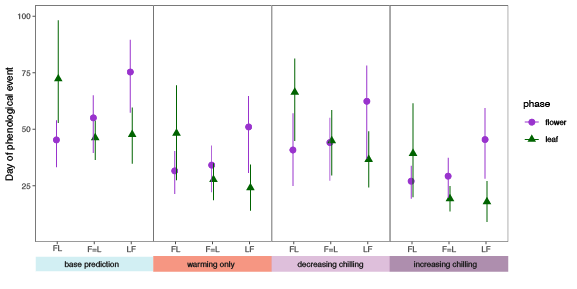
\includegraphics[width=\textwidth]{..//Plots/Flobuds_manuscript_figs/postergroups.png}
 %\caption{Alternative Fig. \ref{fig:preddy}.}
 %\end{figure}

\section*{Figures}
\begin{figure}[h!]
    \centering
         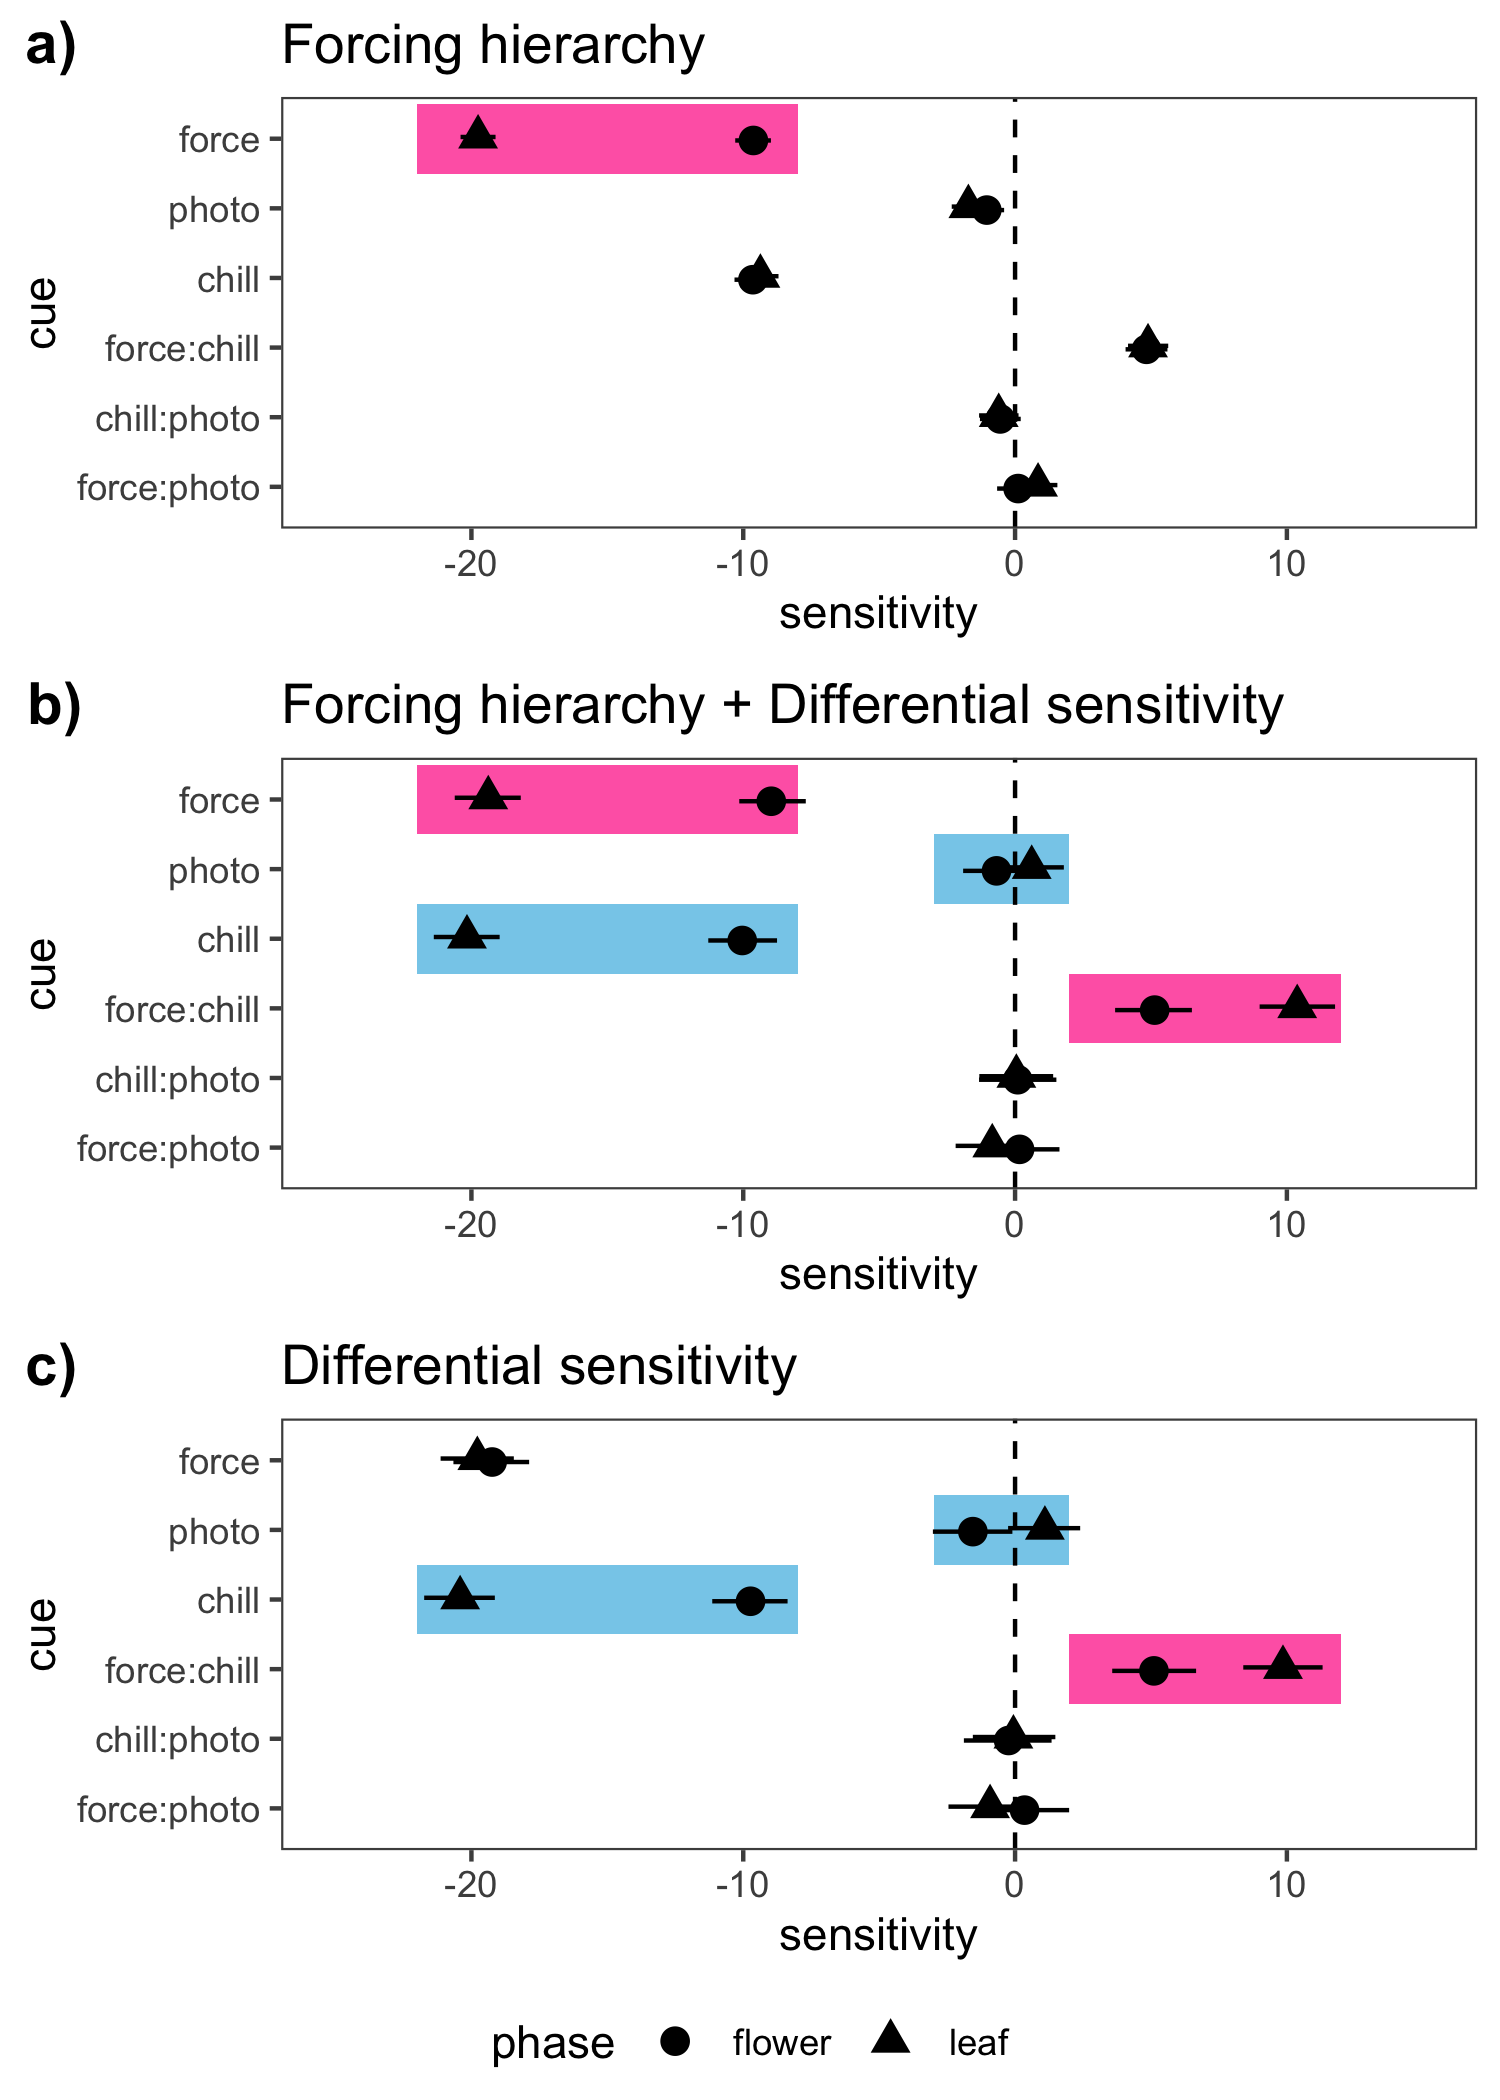
\includegraphics[width=.7\textwidth]{..//Plots/Flobuds_manuscript_figs/simulations.png}
    \caption{Characteristic sensitivity ($\Delta$ day of phenological event/ $\Delta$ environmental cue) patterns of the phenological response to changing cue levels for the two major flower-leaf sequence hypotheses.  \textbf{a)} displays a signature pattern of the forcing hierarchy hypothesis (FHH, pink boxes)---with the second phenophase in the sequence (in this case leafing) having a higher sensitivity to forcing than the first.  \textbf{b)} Highlights a typical sensitivity pattern produced by the differential sensitivity hypothesis (DSH). \textbf{c)} Depicts a scenario where both the FHH and the DSH contribute to flower-leaf sequence variation. Here the characteristic forcing sensitivity of the FHH is still apparent but the differential sensitivity to chilling and photoperiod is seen as well (blue boxes). All plots above are based on simulations (see Supporting Information: Methods). Shapes indicate mean estimates and lines depict 95\% credible intervals from Bayesian hierarchical models with advances in phenology shown as negative numbers, and delays in phenology as positive numbers. } 
    \label{fig:simulations}
\end{figure}
\clearall % EMW5Dec20: Not sure if this will fix the float issue, but it might.

\begin{figure}[h!]
    \centering
         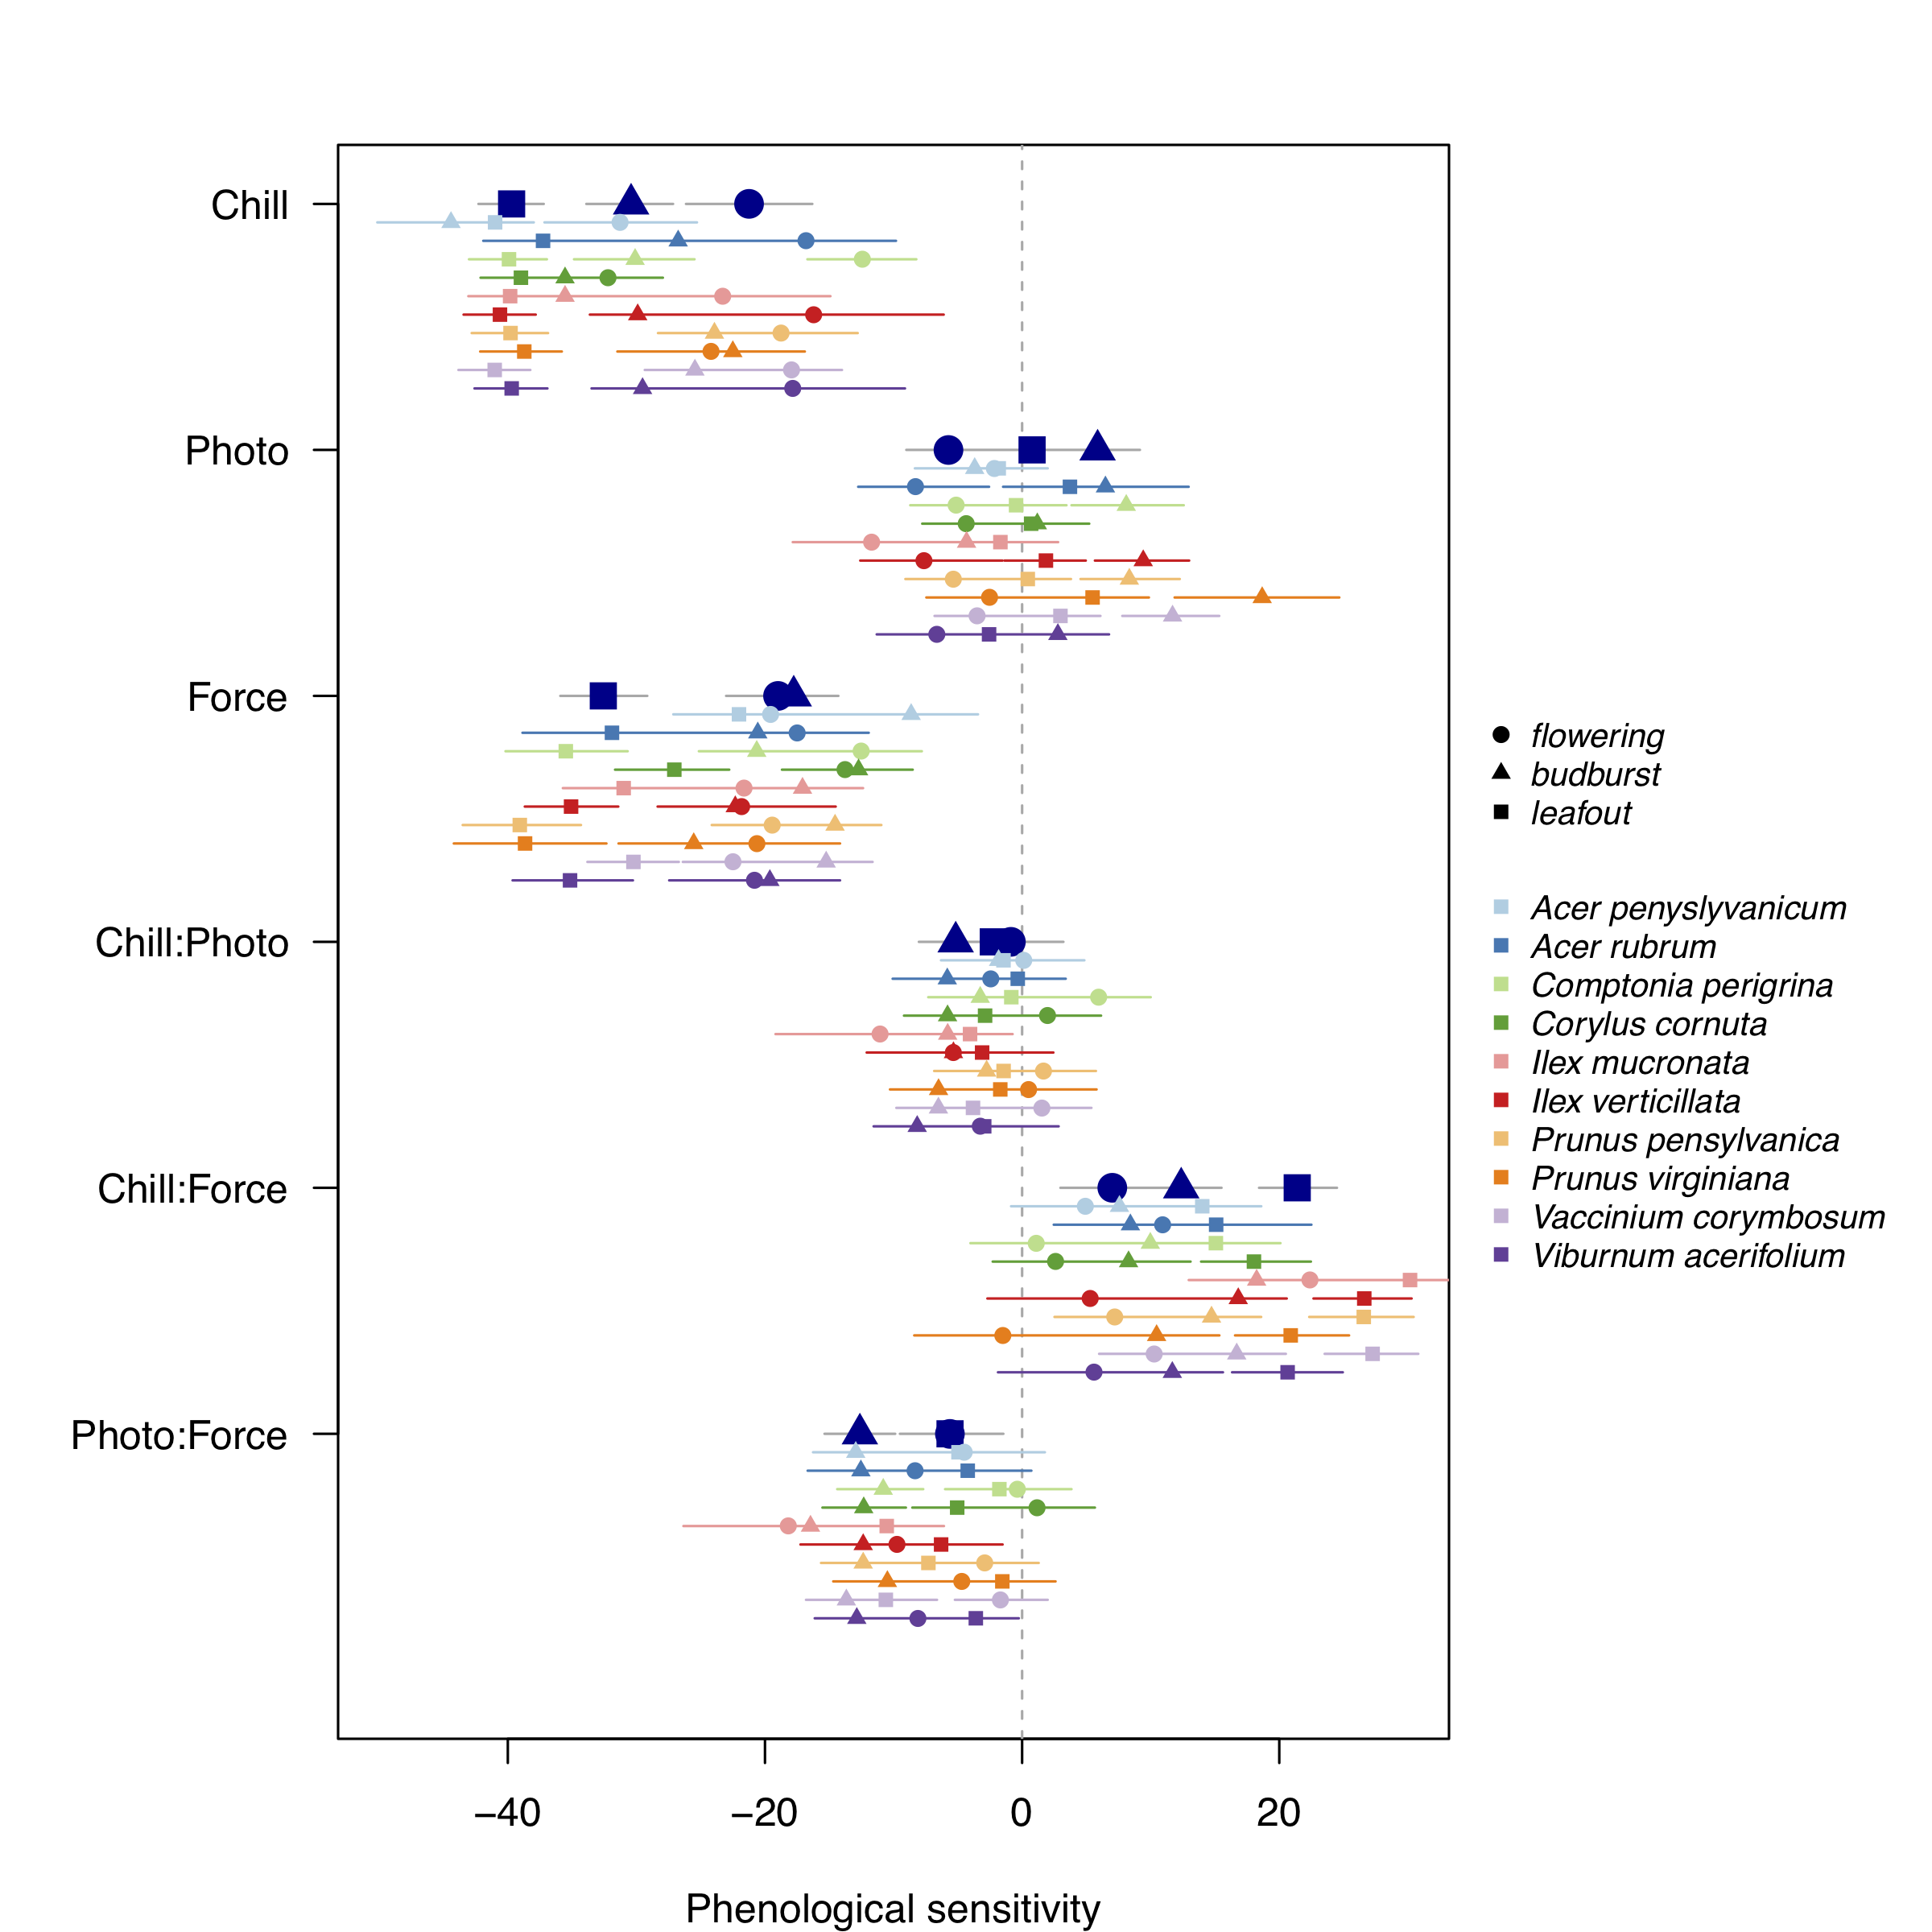
\includegraphics[width=0.9\textwidth]{..//Plots/Flobuds_manuscript_figs/all3phases.png}
         \caption{Effects of forcing temperature, chilling duration, and photoperiod on the leaf budburst (triangles), leafout (squares) and flowering (circles) phenology of 10 temperate woody plant species collected from Harvard Forest (Petersham, MA, USA). Shapes indicate mean estimates and lines depict 50\% credible intervals (See Tab. \ref{tab:modelests}, Tab. \ref{tab:modelests2} for other intervals) from Bayesian hierarchical models with advances in phenology shown as negative numbers, and delays in phenology as positive numbers. Flower and leaf phenology differs in sensitivity ($\Delta$ day of phenological event/ $\Delta$ environmental cue; 4 weeks chilling/6 \degree C forcing/4 hours photoperiod) to these environmental cues. See Fig. \ref{fig:altview} for an alternative presentation of these results that depicts the difference between the mean estimates of each phase (shapes). }
   % \caption{\textbf{Experimental results suggest differential sensitivity to environmental cues between flower and leaf buds}. We used a growth chamber manipulation and Bayesian hierarchical models to evaluate the phenological sensitivity ($\Delta$ day of phenological event/ $\Delta$ environmental cue) of flower and leaf buds to varying forcing temperatures, photoperiods, and duration of chilling.   Vegetative buds (circles) were more sensitive to chilling and cue interactions. Flower buds (triangles) advanced with photoperiod increases under all treatment combinations but leaf phenology was delayed with increasing photoperiod when chilling and forcing levels were low. Points indicate mean estimates and lines represent the 50\% credible intervals. These differential sensitivities dictate how FLS patterns vary with changing environmental conditions.}
    \label{fig:model}
\end{figure}

\begin{figure}[h!]
    \centering
         \includegraphics[width=\textwidth]{..//Plots/Flobuds_manuscript_figs/PHH_plot.png} 
    \caption{Phenological sensitivity ($\Delta$ days of phenological event/ $\Delta$ 6$\degree$C) to forcing temperatures of leaf budburst (triangles) and flowering (circles) phenology from 10 temperate deciduous woody plants at long (12 hour) photoperiod and long chilling duration treatments (8 weeks at 4\degree C). Shapes indicate mean estimates and lines depict 50\% credible intervals (See Tab. \ref{tab:phh} for other intervals) from Bayesian hierarchical models with advances in phenology shown as negative numbers. When photoperiod and chilling are high, most species follows the predicted pattern of the forcing hierarchy hypothesis (FHH), with the second phenophase of the sequence consistently more sensitive to forcing than the first. This result suggests that the FHH should be considered a special case of the differential sensitivity hypothesis (DSH) that occurs when the chilling and photoperiod requirements are met for both tissue types.}
    %\caption{\textbf{Under adequately long chilling duration and photoperiods, the phenological sensitivity ($\Delta$ phenological event/ $\Delta$ C$\degree$) follows the predicted pattern of the forcing hierarchy hypothesis (FHH), with the second phenophase of the sequence consistantly sensitive to forcing as the first.} After performing a growth chamber manipulation evaluate the phenological sensitivity of flower and leaf buds to varying level forcing temperatures, photoperiods, and duration of chilling, we subset out data to include only observation at high chilling and photoperiod levels. Using Bayesian hierarchical models, we quantified the differences in sensitivity to forcing for all species in our study. Points indicate mean estimates and lines depict 50\% credible intervals. Our finding indications that the FHH should be considered a special case of the differential sensitivity hypothesis (DSH) that occurs when the chilling and photoperiod requirements are well met for both bud types.} %emwhalloween20: I think here "Our finding indications that the FHH should be considered a special case of the differential sensitivity hypothesis (DSH) that occurs when the chilling and photoperiod requirements are well met for both bud types." works (though some journals are picky about no conclusions in figure captions, but I like it). 
    \label{fig:FHH}
\end{figure}

\pagebreak

\begin{figure}[h!]
    \centering
 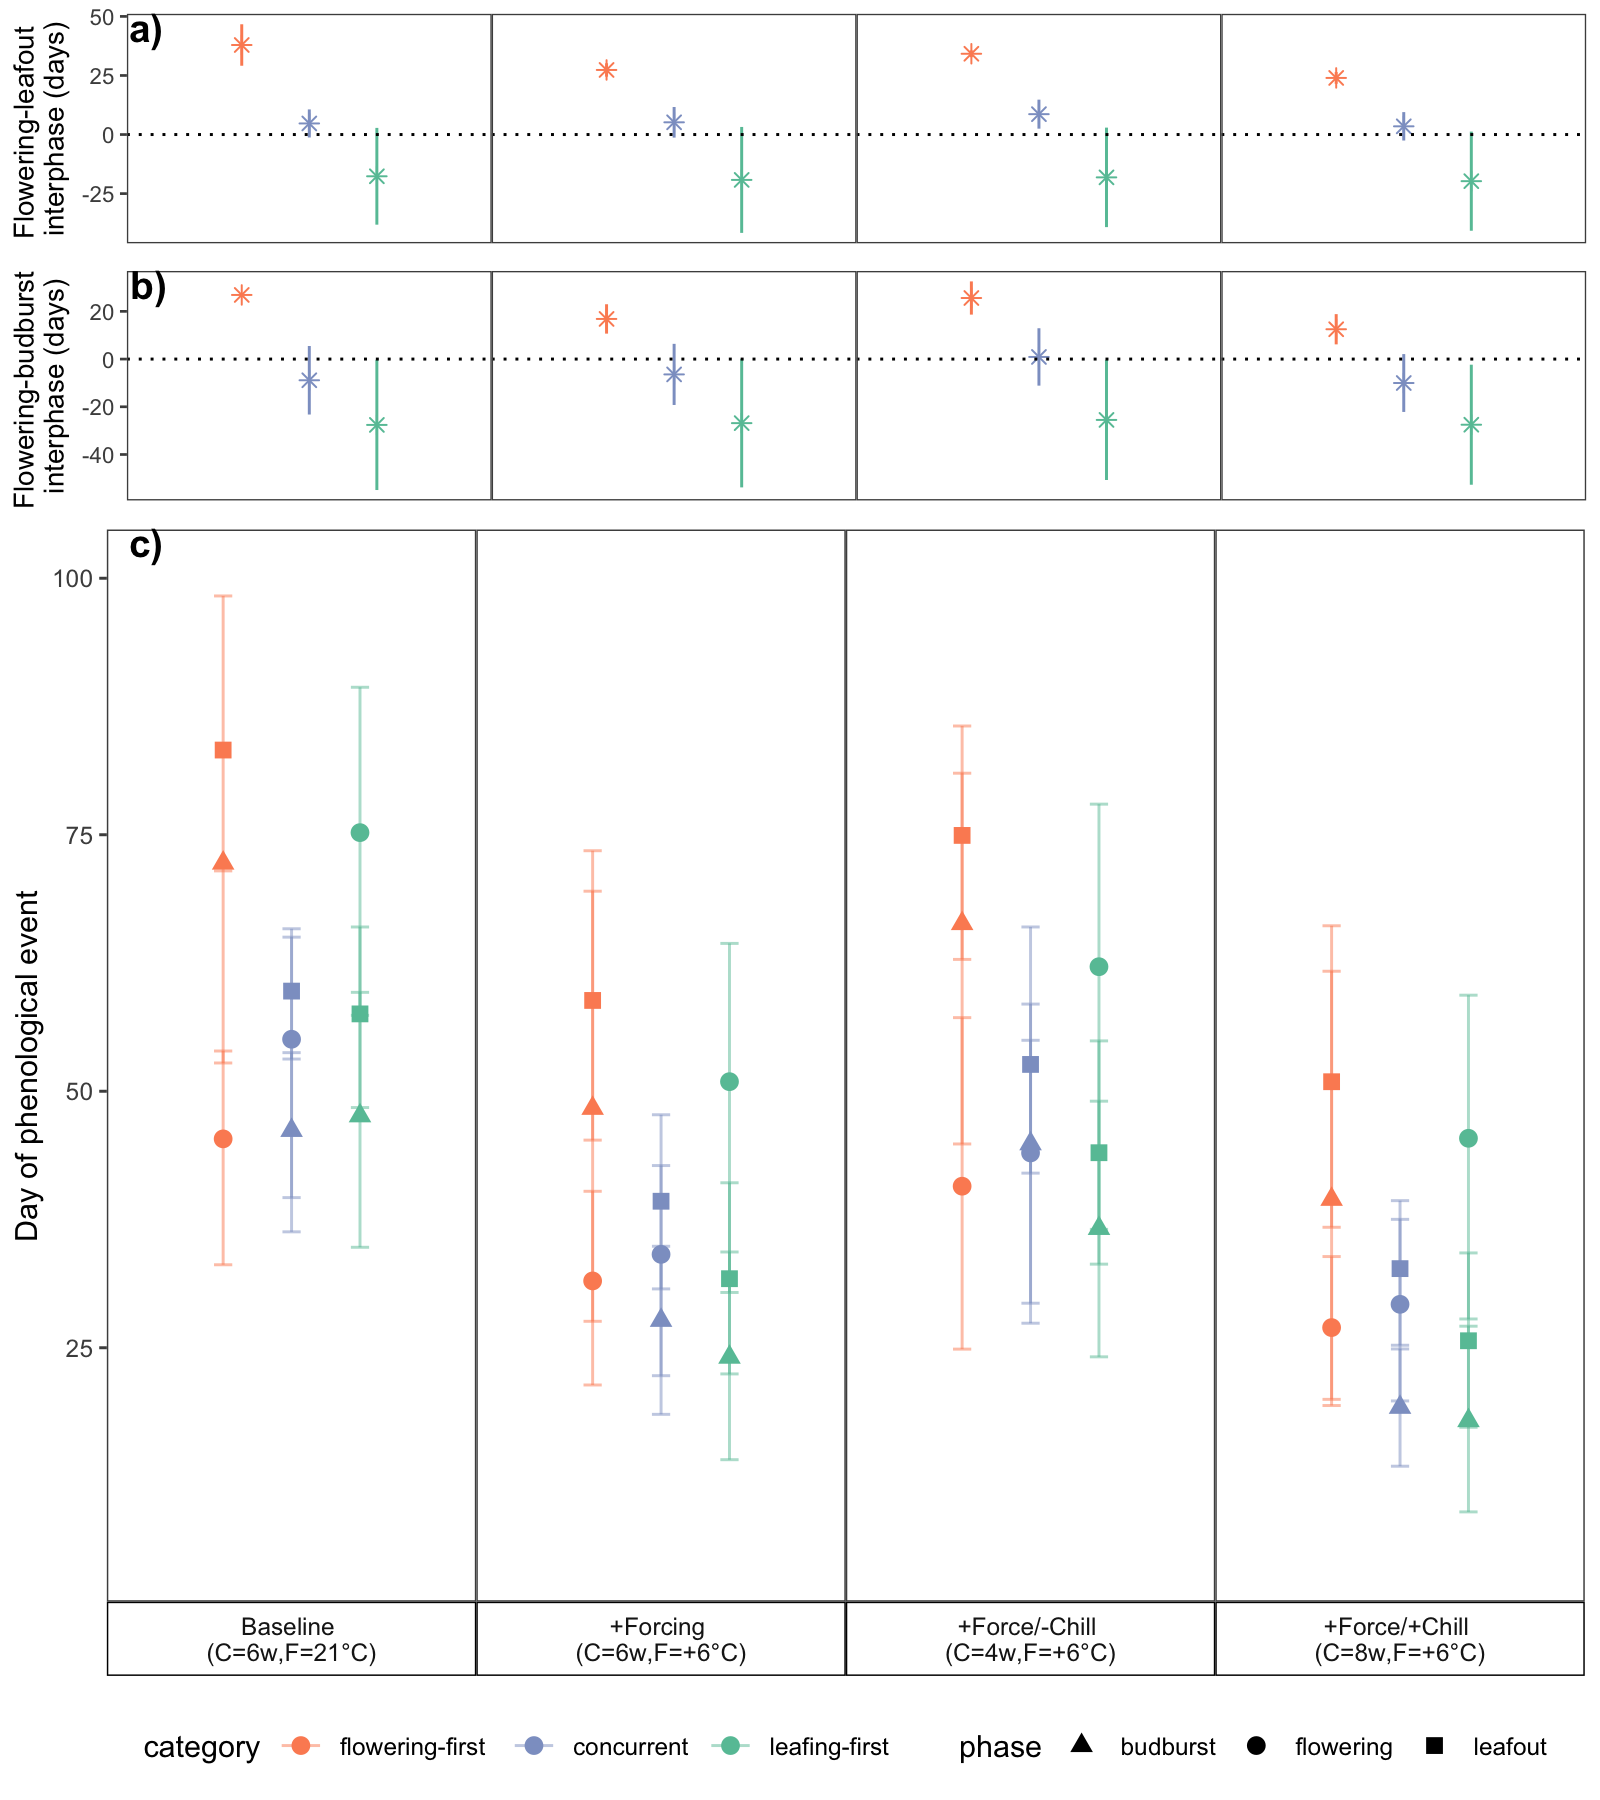
\includegraphics[width=.9\textwidth]{..//Plots/Flobuds_manuscript_figs/posteriorgroups_go.png} 
    \caption{Projected shifts in flower-leaf sequences under current environmental conditions (Baseline) and three climate change scenarios (increase forcing, increase forcing/decrease chilling, increase forcing/increase chilling) predict that FLS shifts differ among the three major FLS types, and will be strongest is flowering-first species. Panels a) and b) show the mean time between flowering and vegetative phenological events (shapes) with 50\% credible intervals (lines). Panel c) shows the predicted event day for each phase. Predictions are based on species-level posterior estimates grouped by FLS category (flowering-first, concurrent, leafing-first) from Bayesian hierarchical models comparing flowering (circles), leaf budburst (triangles) and leafout (squares) phenological responses to variable chilling duration and forcing temperatures. Shapes represent the mean estimates and lines represent the 50\% credible intervals. }
    %\caption{\textbf{Flower-leaf sequences (FLSs) of temperate, woody species will shift with climate change, but the magnitudes of these shifts vary by among FLS categories and depend on the specific dynamics of temperature at a given location.} We used Bayesian, hierarchical models comparing flower and leaf bud responses to variable temperature combinations to predict FLSs patterns under current climate conditions and three climate change scenarios;  an increase in spring warming alone (warm 5), increase in spring warming and increase in winter chilling (warm 5 +chill) and an increase in spring warming and decrease in winter chill (warm 5 -chill). We grouped the species-level posterior estimates by FLS category (flowering-first, concurrent, leafing-first). The points represent the mean estimates and the lines lines represent the 50\% credible intervals. In our study, all flowering-first species are wind-pollinated, and projected FLS shifts are most pronounced in some of these wind-pollinated, flowering-first shrubs. However, FLS shifts for all species depend on the relationship between forcing and chilling changes which is likely to vary by location with climate change.} %emwhalloween20: I like the figure, but need to re-write the caption to highlight species-group differences. 
    \label{fig:preddy}
\end{figure}



\end{document}
